\documentclass[lettersize,journal]{IEEEtran}
\usepackage{amsmath,amsfonts}
\usepackage{algorithmic}
\usepackage{algorithm}
\usepackage{array}
\usepackage[caption=false,font=normalsize,labelfont=sf,textfont=sf]{subfig}
\usepackage{textcomp}
\usepackage{stfloats}
\usepackage{url}
\usepackage{verbatim}
\usepackage{graphicx}
\usepackage{cite}
\usepackage{varioref}
\usepackage{cleveref}
%added xcolor for box color
\usepackage{xcolor}
\usepackage{enumitem}


\hyphenation{op-tical net-works semi-conduc-tor IEEE-Xplore}
% updated with editorial comments 8/9/2021

\begin{document}
	
	\title{Toward Extended Robot Intelligence: Task-Grounded, Memory-Augmented Scene Graphs for Context-Aware and Inclusive Human-Robot Teaming with Multimodal Large Language Models}
	
	\author{Trung Kien La, Saleh Azizpour and Eric Guiffo Kaigom
		% <-this % stops a space
		\thanks{Trung Kien La was with the Frankfurt Industrial Robotics and Digital Twin Laboratory (FriiDA) at the Frankfurt University of Applied Sciences, Hungener Str. 6 Building C, 60389 Frankfurt am Main, Germany (Orcid: 0009-0007-9239-3268).}% <-this % stops a space
		\thanks{Saleh Azizpour is with the Frankfurt Industrial Robotics and Digital Twin Laboratory (FriiDA) at the Frankfurt University of Applied Sciences, Hungener Str. 6 Building C, 60389 Frankfurt am Main, Germany. (e-mail: saleh.azizpour@stud.fra-uas.de).}% <-this % stops a space
		\thanks{Eric Guiffo Kaigom is with the Frankfurt Industrial Robotics and Digital Twin Laboratory (FriiDA) at the Frankfurt University of Applied Sciences, Hungener Str. 6 Building C, 60389 Frankfurt am Main, Germany (e-mail: kaigom@fra-uas.de).}}
	
	% The paper headers
	\markboth{Replace this line with your manuscript id number}%
	{Shell \MakeLowercase{\textit{et al.}}: A Sample Article Using IEEEtran.cls for IEEE Journals}
	
	%\IEEEpubid{0000--0000/00\$00.00~\copyright~2021 IEEE}
	% Remember, if you use this you must call \IEEEpubidadjcol in the second
	% column for its text to clear the IEEEpubid mark.
	
	\maketitle
	
	\begin{abstract}
A future robotized society requires meaningful, context-aware human-robot interactions in which robots actively support human self-determination and well-being. Current systems, however, struggle to follow dynamic human intent, generalize to unseen objects, or communicate their internal reasoning, limiting trust and adoption. To address these challenges, we propose a task-grounded, memory-augmented, human-centered scene graph framework that integrates structured perception, robot-state awareness, and multimodal reasoning via large language models (LLMs). The approach combines semantic object detection with rule- and constraint-based filtering to generate a structured representation of the environment and robot state, enriched with task-specific knowledge and historical interactions through LLM reasoning. This memory-augmented scene graph enables the robot to maintain a persistent context over time, anticipate human needs, and request clarification in ambiguous situations, providing robustness and adaptability to novel tasks. Acting as a human-interpretable interface between perception, reasoning, and interaction, the framework supports navigation, assistance, and guidance through natural language, enabling users to collaborate intuitively with the robot without programming expertise. Scene interpretations can also be delivered via text-to-speech, expanding accessibility and facilitating inclusive human-robot teaming. The system achieved near-real-time object detection at up to approximately 40 FPS and received high perceived usability  in a pilot study with 19 participants across on-site and video-based evaluations. Participants consistently praised the robot's natural and reliable communication, responsive tracking, intuitive and easy-to-use interface, and ability to maintain task context and handle previously unseen objects. These results provide initial evidence that the framework can extend robot intelligence beyond vendor-defined skills toward systems that support human autonomy.
	\end{abstract}
	
	\begin{IEEEkeywords}
		  Mobile robotics, Multimodal LLM, Gemma, YOLO, Scene Graph, Human-robot teaming, Inclusion, Society of the future, pAIrSEEption, 3D scene understanding
	\end{IEEEkeywords}
	
	\section{Introduction}\label{introi}
	
	\begin{figure}[!t]
		\centering
		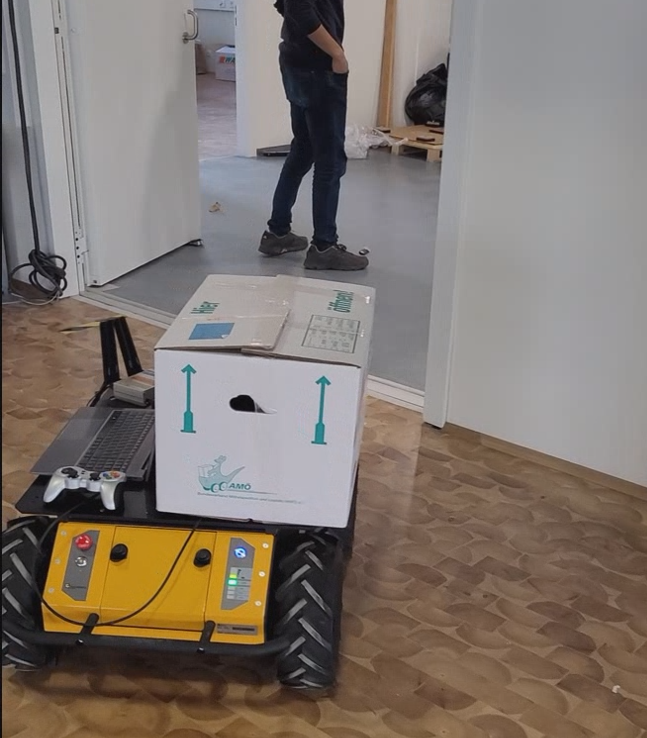
\includegraphics[width=0.9\columnwidth]{pic/movingbox.png}
		\caption{A mobile robot with extended intelligence beyond native, vendor-defined skills. It builds and shares a task-grounded, memory-augmented SG as a mental model to reason about dynamic environments, ensure performance-aware safe navigation, follow verbally expressed human intent, and provide real-time spoken feedback, thereby enabling intuitive, comfortable, programming-free, and inclusive payload transportation.}
		\label{intro}
	\end{figure}

Mobile robots are increasingly deployed in everyday societal applications, such as room cleaning and payload transportation, to relieve humans from repetitive and physically demanding tasks \cite{gona2024intelligent,kaigom2023metarobotics,konnecke2024,la2024toward}. These systems typically rely on predefined rules and task sequences to govern their behavior. However, as robots become more integrated into human-populated and unstructured environments, the variability introduced by human actions and dynamic contexts makes purely static programming impractical \cite{kruger2019programming,ajoudani2018progress,beetz2018knowrob,pedersen2016robotics}. As a result, users often struggle to intuitively instruct robots to interact with entities, such as following a person or approaching objects, especially when these entities are moving or previously unseen.

Traditional solutions often rely on proportional-integral-derivative (PID) feedback control to track the Cartesian pose of detected entities using stereo vision \cite{chen2020vision,wu2021person,li2022robust}. While effective for simple tasks, such approaches lack semantic reasoning capabilities, limiting their adaptability to complex task requirements, unseen situations, and generalization across scenarios.

In this work, we extend this paradigm by combining scene graphs (SGs) for structured environmental representation with multimodal large language models (MLLMs) \cite{gupta2023vlmaps,huang2023vlfm,konishi2023navgpt} for high-level reasoning over hierarchical information. The proposed Extended Robot Intelligence (ERI) framework transforms descriptive situational awareness into actionable knowledge by incorporating persistent contexts, objectives, and constraints into the representation. This enables intuitive human-robot interaction through natural language, removing the need for technical expertise and promoting inclusion. Furthermore, using shared semantic representations improves the transparency of robot decision-making, allowing users to better understand, anticipate, and influence robot behavior.

%The main contribution is not merely generating scene descriptions with an MLLM, but constructing a task-grounded and memory-augmented scene graph that fuses object detections, 3D spatial attributes, robot-state information, task constraints, and interaction history for context-aware mobile robot behavior.

Our main contributions are as follows:


\begin{itemize}
	\item Task-grounded and memory-augmented SG: 
	We construct SGs that go beyond MLLM-based scene description by fusing object detections, 3D spatial attributes, robot-state information, task constraints, and interaction history into a persistent representation for context-aware mobile robot behavior.
	
	\item Hybrid perception-to-semantic-awareness pipeline: 
	We combine deterministic preprocessing, rule- and constraint-based filtering, and MLLM reasoning to transform object-level perception into task-relevant, human-interpretable representations that support intuitive understanding, user self-determination, safe navigation, assistive interaction, and ambiguity handling.
	
   \item Human-centered, resource-efficient interaction:
We develop a voice-driven interface that generates SGs on demand from single frames. Through natural-language text-to-speech feedback, the interface enables intuitive, programming-free interaction, supports user self-determination, and remains deployable on resource-constrained robotic platforms.
\end{itemize}

The remainder of this paper is organized as follows. Related work is presented in \cref{relatedwork}. The proposed method and its implementation are described in \cref{methodology}. The experimental results are presented in \cref{sec:experiments}. Finally, \cref{conclusion} concludes the paper.


\begin{table*}[!hb]
	\centering
	\caption{Tools and models for 3D SGG, perception, navigation and interfacing in robotics}
	\label{tab:scenegraph_technologies}
	\resizebox{\textwidth}{!}{%
		\begin{tabular}{|l|l|l|l|l|}
			\hline
			\textbf{System/Framework} & \textbf{\begin{tabular}[c]{@{}l@{}}Detection \& Segmentation \\ (Nodes)\end{tabular}} & \textbf{\begin{tabular}[c]{@{}l@{}}Semantic Features \& \\ Embeddings\end{tabular}} & \textbf{\begin{tabular}[c]{@{}l@{}}Relation Inference \& \\ Planning (Edges)\end{tabular}} & \textbf{\begin{tabular}[c]{@{}l@{}}Alternatives \& \\ Additional Models \& \\ Misc. \end{tabular}}  \\ \hline
			\textbf{ConceptGraphs}\cite{conceptgraphs} & SAM & CLIP, Grounding DINO & GPT-4, LLaVA & RAM \\ \hline
			\textbf{3DGraphLLM}\cite{3dgraphllm} & Mask3D, OneFormer3D & DINOv2 (2D), Uni3D (3D) & VL-SAT, CLIP & LLaMA3-8B, Vicuna-1.5 \\ \hline
			\textbf{Graph2Nav}\cite{graph2nav} & PSGFormer, Mask2Former & Panoptic Labels & 2D-PSG Inference, GPT-3.5 & LIO-SAM, Whisper \\ \hline
			\textbf{HOV-SG}\cite{hovsg} & SAM & CLIP & Hierarchical Heuristics & GPT-3.5, GPT-4 \\ \hline
			\textbf{OpenIN}\cite{openin} & CropFormer & SBERT, CLIP & GPT-4o & Tokenize Anything \\ \hline
			\textbf{SG-Nav}\cite{sgnav} & SAM & VLMs, LLMs & LLaMA-7B, GPT-4, LLaVA & Fast Marching Method \\ \hline
			\textbf{Interaction Updates}\cite{interaction} & Existing 3D SG (e.g., Hydra) & Visual Transformer (ViT) & GPT-4, BLIP-2 & DBSCAN (Denoising) \\ \hline
			\textbf{VisionGPT}\cite{visiongpt} & YOLO-World & Proportional 2D Coordinates & GPT-3.5 Turbo, GPT-4 & H-Pattern Splitter \\ \hline
			\textbf{LGX}\cite{lgx} & GLIP, YOLO & BLIP (Captions) & GPT-3 & OWL-ViT, Detectron2 \\ \hline
			\textbf{VLMaps}\cite{gupta2023vlmaps} & LSeg & CLIP & Codex (Code-writing LLM) & RTAB-Map \\ \hline
		\end{tabular}%
	}
\end{table*}


\section{Related Work}\label{relatedwork}
Societal applications typically take place in unstructured environments, such as homes, where multiple objects exhibit spatial, temporal, and contextual dynamics. These changes can arise from uncertain human activities as well as from the appearance and disappearance of entities with specific properties and affordances in the 3D scene \cite{yalcinkaya2024towards}. SGs provide a structured and multimodal representation of the sensed environment, allowing robots to reason about their operational space and generalize appropriate actions. Neural-network-based approaches have therefore been proposed for object detection, scene graph generation (SGG), and interpretation in mobile robotics. The following subsections review relevant methods for SGG and outline their connections to our approach.

\subsection{Scene Graph}\label{scenegraph}

An SG represents a scene in a structured form by encoding objects, their attributes, and relationships. SGG can be derived from images, text, or videos. An SG is a hierarchical graph consisting of nodes $O$ and edges $E$. Nodes represent objects such as humans or items (e.g., bicycle, car), as well as parts of objects (e.g., a person's arm). Each node may include attributes describing the object's state, such as color, size, or pose. Edges often represent relationships between object pairs, describing actions (e.g., man holds cup) or spatial relations (e.g., man stands in front of bench). These relationships are typically expressed as triples 
$\langle \text{subject} - \text{predicate} - \text{object} \rangle$ \cite{li2024scene}.
\subsection{Tools for Scene Graph Generation}
\noindent Various models and technologies are used for SGG across robotics, computer vision, autonomous navigation, and human-machine interaction (see Table~\ref{tab:scenegraph_technologies}). Recent advances in Foundation Models have shifted the field from class-limited object recognition toward universal segmentation models (e.g., Segment Anything Model (SAM/SAM2)~\cite{jiaxing2025sam2}) and open-vocabulary encoders such as Contrastive Language–Image Pretraining (CLIP)~\cite{chen2024clip}, which provide pixel-accurate masks and semantic embeddings. These capabilities allow modern MLLMs and Vision-Language Models (VLMs) to recognize not only object classes but also semantic states and complex relationships. Frameworks such as ConceptGraphs~\cite{gu2024conceptgraphs} and 3DGraphLLM~\cite{zemskova20253dgraphllm} leverage this information to construct SGs interpretable for LLMs while grounding objects in 3D space using geometric data from sensors such as Light Detection and Ranging (LiDAR) or depth cameras. 

Other approaches, including VLMaps~\cite{huang2023visual} and Graph2Nav~\cite{shan2025graph2nav}, translate these spatial relations directly into navigation commands. Many existing frameworks require prior mapping or 3D reconstruction \cite{3dgraphllm,hovsg,openin,interaction}, while others construct maps online in previously unknown environments \cite{conceptgraphs,graph2nav,sgnav,lgx,gupta2023vlmaps}. However, such approaches typically depend on powerful hardware, multiple sensors, and extensive preprocessing, often involving LiDAR or depth-based scanning of entire environments. The resulting maps are then enriched with semantic descriptions, for instance through MLLMs, enabling tasks such as visual question answering about specific objects. In contrast, our approach aims to be resource-efficient and cost-effective. It generates a SG directly from the current image only when needed (e.g., to describe the scene), avoiding time-consuming mapping and enabling dynamic operation.

\subsection{Layered Architecture for Scene Graph}

Mobile robots can reason over contextualized and structured information to plan and achieve goals. Recently, SGs have been adapted for mobile robotics, and multiple abstraction layers of real-world scenes have been introduced for this purpose. These include the spatial layer, which represents locations within the scene; the semantic layer, which captures the meaning of entities, including their states, affordances, predicates, and other attributes; the topological layer, which represents connectivity between locations; and the task-related layer, which encodes robot goals \cite{rana2023sayplan,im2024egtr}. Entities  in the scene populate these layers, which differ in several respects. One such distinction is the update rate of entity attributes \cite{rana2023sayplan,im2024egtr}. For example, the robot initial and final positions may be known in advance and can therefore be treated as fixed, whereas task completion may be required within a short time window, prompting the robot to execute motions more quickly. In contrast, in entity-following applications, the robot desired position changes over time, indicating a dependence of the scene perception on the task and robot dynamics  often omitted.


\begin{figure}[!t]
	\centering
	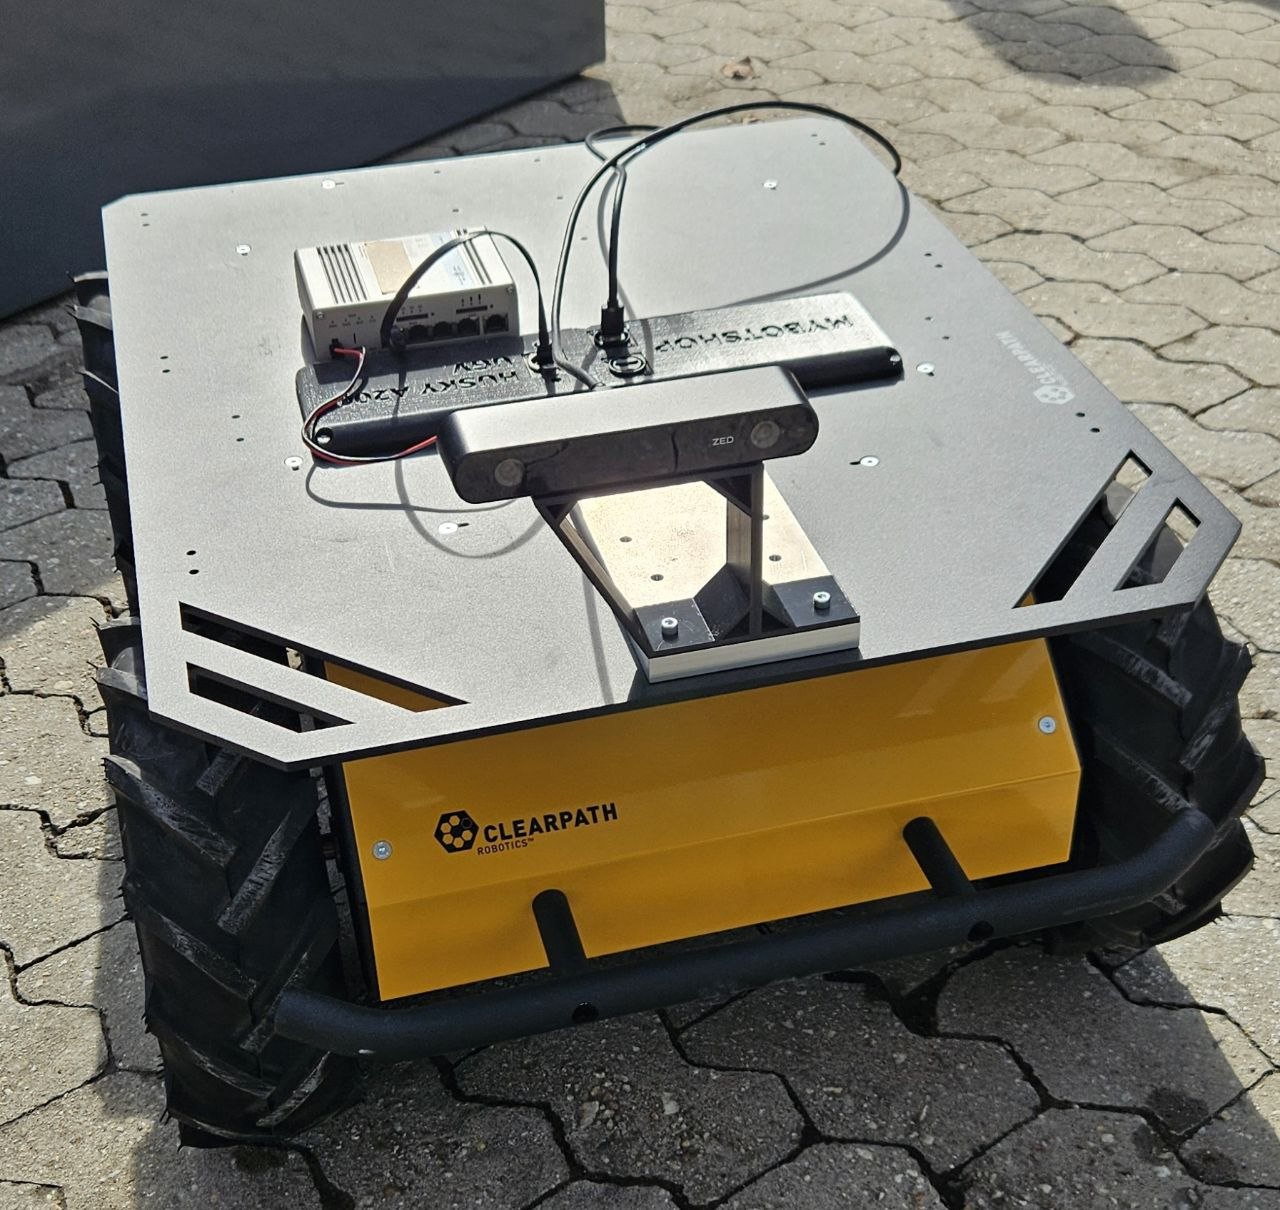
\includegraphics[width=2.2in]{images/husky_zed.jpg}
	\caption{Husky Robot as a mounting platform for the ZED 2i camera.}
	\label{husky_robot}
\end{figure}

In this work, to ensure task relevance and physical feasibility, we employ a hybrid rule- and constraint-based filtering layer coupled with MLLM reasoning. Rule-based components encode spatial, semantic, and task-specific knowledge (e.g., distance thresholds, motion classification, and target selection), while constraint-based components enforce feasibility conditions such as safety, kinematics, and perception confidence. The resulting structured and task-grounded representation is used to construct a prompt for the MLLM, which performs high-level semantic reasoning. This allows the model to infer task-relevant relationships, resolve ambiguities, and generate human-interpretable scene descriptions. By combining rule-based pre-processing, constraint enforcement, and MLLM reasoning, the system produces a dynamic SG that is both semantically meaningful and operationally valid for real-world robotic tasks. Unlike purely rule-based SGs, our hybrid approach enriches the SG with conversation history and task-related experiences, resulting in a memory-augmented representation. Using the profile history to anticipate object affordance and actions enhances  user experience.

\begin{comment}

  \begin{table}[!t]
	\centering
	\caption{Classification of  Algorithms and Inference Concepts for SGG.}
	\label{tab:features}
	\begin{tabular}{|c|c|c|c|}
		\hline
		\textbf{Source} & \textbf{Feature representation} & \textbf{Method for relation inference} \\
		\hline \hline
		\cite{kim2025semantic,su2024adopting} & Box-based &  MPNN, CNN    \\
		\hline
		\cite{im2024egtr,hao2025bctr} & Query-based &  Attention mechanism  \\
		\hline
		\cite{liu2021fully,newell2017pixels} & Point-based &  CNN \\
		\hline
	\end{tabular}
\end{table}

	Inhalt...
\end{comment}

%\subsection{Algorithms for the generation of scene graphs}
%Three main classes of feature representation and  relation inference have emerged in SGG (see \cref{tab:features}). Semantic SGG has recently shifted the focus from object- to relation-centric to handle multi-object relationships in real scenes \cite{kim2025semantic}. The approach combines object detection based on a fast Region-based Convolutional Neural Network (R-CNN), an edge-dual scene graph, and an object-relation-centric Message Passing Neural Network (MPNN). The MPNN aggregates information from neighboring entities to learn object- and relation-centric features, enabling iterative updates of entity representations and producing a feature vector for the entire graph \cite{kim2025semantic,su2024adopting}. Recent SGG approaches also exploit attention mechanisms by connecting objects with significant attention weights derived from the self-attention layers of a pre-trained DEtection TRansformer (DETR) \cite{im2024egtr}. A third strategy is Convolutional Scene Graph Generation (CSGG), where objects are encoded as bounding-box center points and relationships are represented as 2D vector fields pointing from subject to object \cite{liu2021fully}. Key characteristics of these approaches are summarized in \cite{liu2024repsgg} and reported in \cref{tab:features}.  We use a box-based approach (YOLO (You Only Look Once), CNN) and extend it with an MLLM to determine relations between objects. To this end, we combine a deterministic preprocessing (see Fig. \ref{transformation_template}), natural language, and logical inference to enable societal robot reasoning.


%\subsection{Tools for the genereration of scene graphs}

%Different tools have been developed to perform the intermediate operations required for SGG from sensed data. An overview of these tools is presented in \cref{tab:scenegraph_technologies}. For example, YOLO and SAM (Segment Anything Model) play key roles in object detection and segmentation tasks. SAM is a general-purpose model capable of performing pixel-level segmentation, whereas YOLO primarily provides bounding-box detection. YOLO is specifically optimized for low latency, making it suitable for real-time scenarios in dynamic, human-centered environments where rapid collision avoidance is critical. This enables faster collision handling while the system follows human motion paths within our framework. CLIP is widely used for extracting semantic features due to its open-vocabulary capabilities. It supports multimodal classification at both the pixel and bounding-box levels. The shared semantic embedding space provided by CLIP enables a seamless transition from image-based perception to language-driven understanding, for example through GPT-based prompting.


\subsection{Operationalization  of Scene Graphs}
SGs have been used in  societal applications, such as finding seating in indoor environments \cite{ravichandran2025safety}, assisting with cooking \cite{kwon2025large}, and supporting city-scale inspection missions \cite{viswanathan2024xflie,amiri2022reasoning}. However, most SGs are constructed from single images, whereas human activities typically span longer time horizons. To address long-term goals, \cite{ravichandran2025safety} federates local SGs from successive images into a global SG. In contrast, our approach leverages an MLLM that exploits reasoning history and generalization capabilities for long-term reasoning. Similar contextual grounding is explored in \cite{kwon2025large} using the generative capabilities of an LLM. We extend this scene-centered contextualization by considering internal robotic processes, including sensed kinematic behavior, motion dynamics, and predicted energy consumption. Our framework thereby unifies scene awareness,  motion planning, and feasibility assessment. By leveraging AI-based SGs and MLLMs, the robot achieves enhanced visual and semantic awareness of the environment, including areas not directly perceived by human teammates. We define this novel capability, which bridges scene-level \textit{perception} and system-level introspection through MLLM reasoning, as \textit{pAIrSEEption}. This capability enables the robot to assist and guide humans in real-world applications via natural spoken language. Its key components are illustrated in~\cref{overview_framework}.

\begin{figure}[!t]
	\centering
	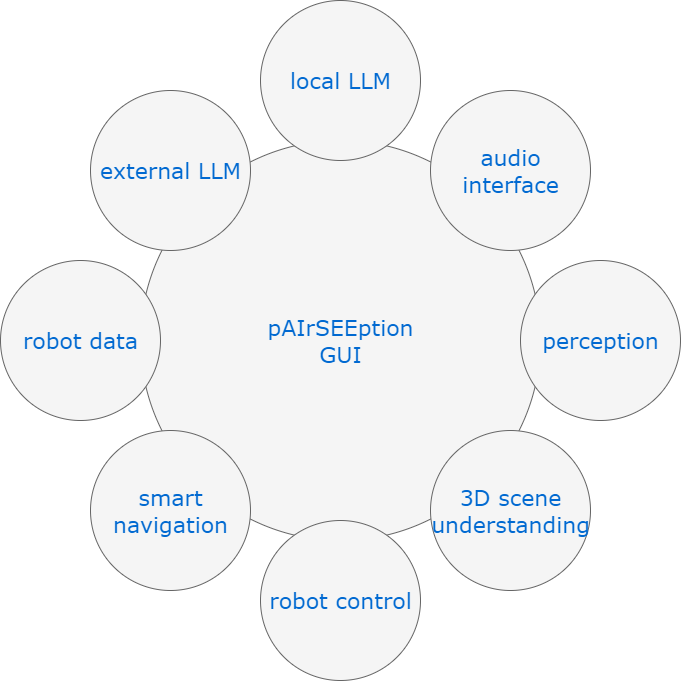
\includegraphics[width=2.4in]{images/overview_eng.png}
	\caption{Features and components of the pAIrSEEption functionality.}
	\label{overview_framework}
\end{figure}

\section{Methodology}\label{methodology}
%This section presents  developed methods and their implementation. 

\subsection{Overview of Features and Components}

\textit{pAIrSEEption} provides a multi-modal access to the  perception, reasoning, and introspection of the robotic system, aligned with human perceptual modalities such as vision, hearing, and speech through AI-driven integration. At its core, it leverages a memory-augmented SG that integrates structured environmental and robot-state information with past interactions and task experience. This enables natural, context-aware human-robot teaming for assistance and guidance without requiring users to write code. Live audio feedback, visual awareness of the environment, and monitoring of the robot’s intentions and predicted performance can be dynamically customized through the responsive GUI in Fig.~\ref{framework_architecture}. By grounding interactions in the SG’s memory via MLLM reasoning, \textit{pAIrSEEption}  provides continuity, adaptability, and robustness to perception uncertainty and evolving task contexts.

The GUI is platform-independent. It can be deployed on different devices, such as the  Jetson AGX Orin (32\,GB) edge platform onboard or a standard laptop with  integrated Nvidia GPU. A ZED~2i stereo camera is connected to these devices for perception. Its wide $110^\circ\text{(H)}\times70^\circ \text{(V)}\times120^\circ \text{(D)}$  field of view is used to capture context-relevant details beyond the user’s line of sight, while providing robust performance under varying lighting and texture conditions. The PID-controlled mobile Husky UGV robot~\cite{husky} is the mounting platform for  hardware components (see Fig.~\ref{husky_robot}). The GUI serves as  visualization and control center of the system, where all  data streams are integrated. The interface displays the following information:







\begin{itemize}
	\item A live annotated stereo-camera video stream from the perception pipeline. 
	\item System performance statistics, such as frames per second (FPS) and utilization of  CPU, GPU, VRAM, and RAM.
	\item Status and system messages indicating active or inactive processes.
	\item Transcribed user voice commands for quality check.
	\item Scene descriptions and conversational responses generated by the LLM based on object data and current images.
	\item Navigation control for selecting detected objects to follow or approach, simplifying target selection even remotely.
	\item Internal robot diagnostics (e.g., motor temperatures) queried via voice commands and displayed in the GUI.
\end{itemize}

Displayed data, along with user voice inputs, can be stored locally in common file formats through the GUI. This enables dataset collection for potential future fine-tuning or training of the YOLO (You Only Look Once) and MLLM models.




\begin{figure*}[!t]
	\centering
	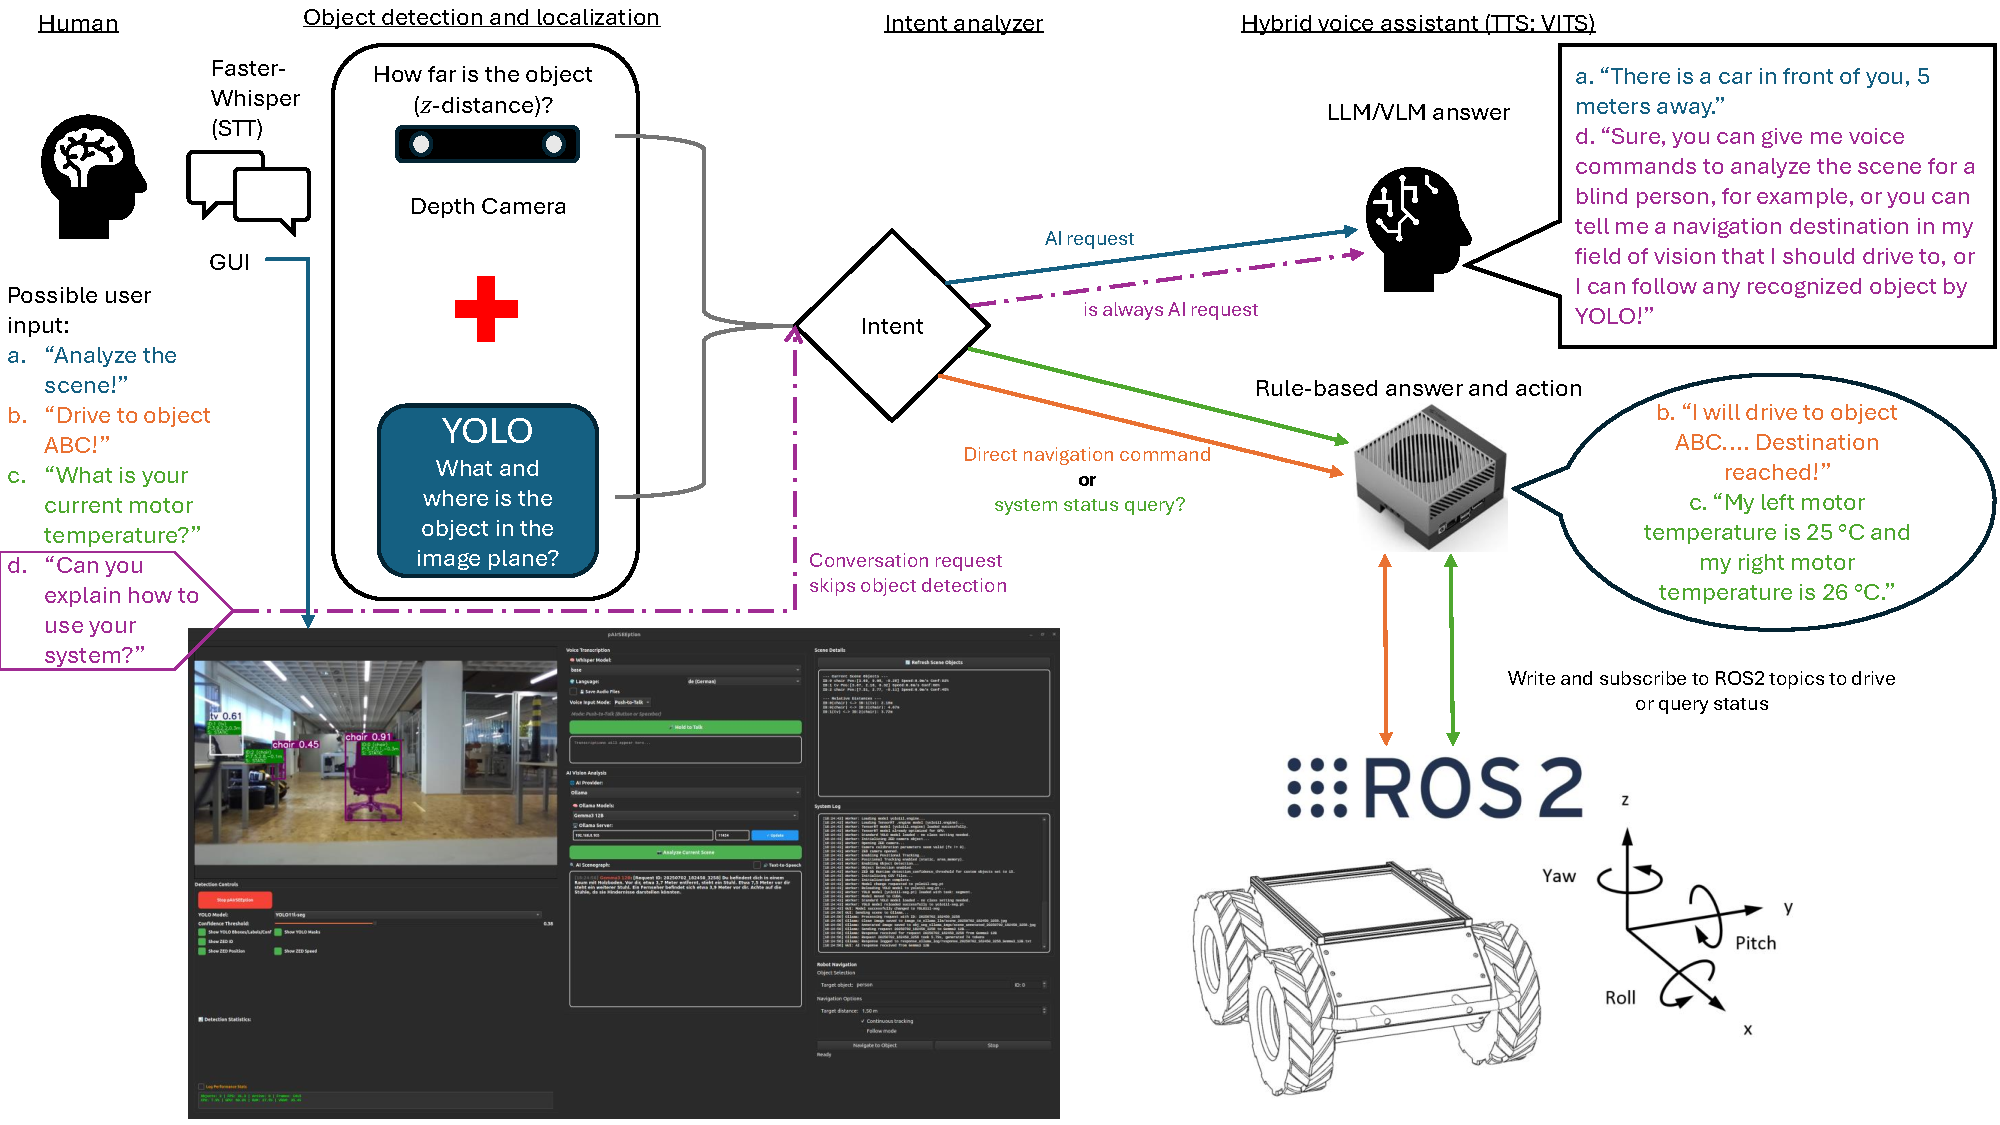
\includegraphics[width=\textwidth]{images/framework_architecture.pdf}
	\caption{System components and data processing pipeline (reading from left to right).}
	\label{framework_architecture}
\end{figure*}

\subsection{Data Processing Pipeline}

The interface provides multiple versions and sizes of YOLO and YOLOE (open-vocabulary) models for object detection and segmentation, as well as MLLMs for scene interpretation. These options can be extended as needed. The GUI also allows configuration of YOLO parameters, including the display of bounding boxes, classification labels, and confidence values. A confidence slider enables filtering of detections below a selected threshold.

The data flow throughout the system is organized into five layers (see Fig.~\ref{framework_architecture}, reading from left to right):


\begin{enumerate}
	\item Voice (speech-to-text, STT) or text input via the GUI (e.g., scene description, navigation goal, robot status, or casual conversation).
	\item Object detection with distance estimation. This step is skipped when a purely conversational interaction with the MLLM is requested.
	\item Preprocessing through a rule-based intent analyzer that determines the requested task. Although this component could be replaced by a lightweight LLM orchestrator, the rule-based approach offers lower latency and greater resource efficiency, which is important in time-critical scenarios.
	\item Hybrid response generation via either the MLLM or predefined rule-based messages. All responses are communicated through the text-to-speech (TTS) system. Scene descriptions and conversations are handled by the MLLM, while robot status queries and navigation commands (e.g., following or approaching an object) are processed through rule-based logic.
	\item When navigation or system status is requested, the system publishes or subscribes to ROS2 topics to control the robot or retrieve status information.
\end{enumerate}


\subsection{Task-Grounding and Memory-Augmentation} \label{SGmemory}
Efficient YOLO-based object detection serves three purposes in the system. First, YOLO provides real-time 2D detections that are fused with ZED~2i depth measurements via the ZED SDK to estimate spatial object information (e.g., distance and 3D position; see Fig.~\ref{framework_architecture}). These data are then formatted (Fig.~\ref{transformation_template}) and passed to the MLLM as part of the grounded input prompt. Second, although modern MLLMs/VLMs can generate 2D bounding boxes, YOLO is employed as a lightweight preliminary detection layer to reduce the computational load on the MLLM and minimize inference latency. Third, the detections enable navigation and object-following. For this purpose, the distance between each detected object and the camera, as well as pairwise inter-object distances within a frame, are computed using the 3D Euclidean metric. The target object is selected through its unique identifier (ID), which can be specified either by voice input or via the graphical interface.

In \textit{pAIrSEEption}, scene objects (e.g., a detected stationary person) are represented schematically as follows:





\begin{equation}
	\begin{aligned}
		o_1 = \Bigl(\text{person},\ 
		\left\{
		\begin{aligned}
			& \text{ID} = 1, \\
			& \text{confidence value} = 0.95, \\
			& \text{3D position} = (x, y, z), \\
			& \text{3D speed} = (v_x = 0, v_y = 0, v_z = 0), \\
			& \text{speed classification} = \text{static}
		\end{aligned}
		\right\}
		\Bigr)
	\end{aligned}
	\label{eq:o1}
\end{equation}
The object $o_1$ is assigned  attributes ID, confidence score, 3D position, 3D velocity, and the classification \textit{static} if the velocity is zero. The object data are expressed in the depth-camera reference frame; thus, the estimated 3D position ($x,y,z$) and velocity ($v_x,v_y,v_z$) are defined relative to the camera.

The GUI supports different MLLMs and distinguishes between locally hosted and cloud-based models accessed via OpenRouter. Local models (e.g., through Ollama), such as Gemma~3 or Qwen~2.5~VL, can run on consumer PCs or edge devices like the Jetson Orin, depending on model size. Gemma~3 supports multimodal input with a large context window and improved attention to small visual details, while Qwen~2.5~VL is often preferred for accurate captions, particularly when text appears in images (OCR). Both models support multilingual interaction and offer multiple quantization options~\cite{gemma3,qwen25vl}. Running models locally provides advantages such as data privacy, version control, and offline operation, but requires suitable hardware. Quantized or specialized models can also be deployed on weaker hardware. Alternatively, cloud-hosted models can be accessed through the OpenRouter API, which enables connections to various models from providers such as OpenAI, Google, Meta, and Anthropic. While these models typically require payment per request and depend on server availability, they reduce local hardware requirements because inference runs on external servers.
To accommodate both scenarios, the system implements a client-server architecture (REST API). Images and merged object data are transmitted from the GUI to the MLLM server as part of the prompt. The server processes a single image together with object speed information, allowing the MLLM to infer whether objects are moving or stationary. Without this additional information, motion cannot be determined from a single frame. Processing single images instead of multiple frames reduces computational load and prevents excessive requests to the MLLM. For instance, the following prompt instructs the MLLM to analyze the data and generate a scene description for safe navigation of visually impaired users:
\noindent
\begin{center} 
	\fcolorbox{black}{black!5}{%
		\begin{minipage}{0.92\columnwidth}
			\setlength{\parskip}{0.5em}
			\ttfamily
			
			Describe the image briefly and precisely using the object data provided.
			
			\{object\_description\}
			
			Describe what can be seen in the image,
			where important objects are located,
			and provide information about possible obstacles.
		\end{minipage}%
	}
\end{center}

\begin{figure}[!b]
	\centering
	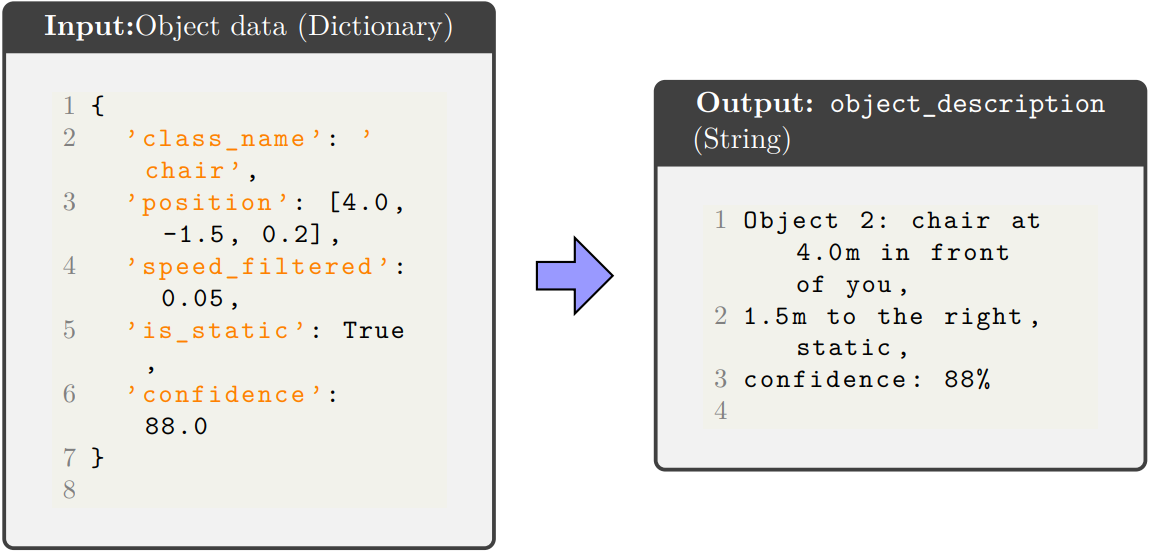
\includegraphics[width=\columnwidth]{images/transformation_template.png}
	\caption{Data preprocessing: Transformation of object data into a readable description for prompt input.}
	\label{transformation_template}
\end{figure}

The object data, defined as \textit{object\_description}, are included in the prompt and converted into concise bullet points during preprocessing. Initially, a template was employed to structure the raw data. Fig.~\ref{transformation_template} illustrates the result of this deterministic transformation. By combining structured object data with image inputs, the MLLM generates a human-readable description of the 3D scene, as demonstrated in Fig.~\ref{transformation_template}. \textcolor{black}{Unlike traditional perception-only pipelines, the  SG is constructed by enriching and fusing  detected and structured object data along with robot-state information with MLLM-generated semantic and task-grounded properties, forming a memory-augmented SG. These outputs are stored as CSV and text files, creating a local structured memory that allows the system to maintain context over time and request clarification in ambiguous situations. An  example is when multiple objects of the same class (e.g., cars) appear in the scene.} Integrating structured perception, memory, and reasoning enables context-aware, human-guided interaction, marking a significant advancement over conventional SG approaches.




The generated scene interpretation is displayed in the GUI output window and can optionally be played back using the TTS system. This integration of a memory-augmented SG with MLLM reasoning and multi-modal interaction yields several advantages with far-reaching societal impact. For example, such functionality can assist blind or visually impaired users during navigation, providing context-aware guidance that adapts to dynamic environments. Beyond accessibility, this extended robot intelligence enables intuitive human-robot collaboration by allowing users to understand, monitor, and interact with the robot’s internal reasoning in real time. 

%Symbiotic and robust human-robot teaming emerges as the robot leverages task-grounded, memory-augmented reasoning to anticipate human needs and adapt to uncertain or ambiguous situations, while the human continuously shapes the robot’s behavior through real-time interaction. %An example of  semantic scene interpretation is presented in Section~\ref{subsec:sceneunderstanding}.





\section{Evaluation and Results}
\label{sec:experiments}

This section presents hardware test results and benchmarks obtained using YOLO models integrated into \textit{pAIrSEEption}, as well as the inference times of MLLMs such as Gemma~3 and Qwen~2.5~VL for generating scene descriptions. The second experiment reports results from two usability evaluations focusing on human-robot interaction and object-following tasks.

\subsection{Performance of YOLO-based Perception}

The average frames per second (FPS) and GPU utilization for several YOLO models of different sizes integrated into \textit{pAIrSEEption} are shown in Fig.~\ref{fig:yolo_comparison}. FPS is a key metric for evaluating the perception module because it directly affects system responsiveness, navigation accuracy, tracking performance, and overall operational safety.
The framework supports YOLO models in PyTorch (\textit{.pt}), \textit{.onnx}, and TensorRT (\textit{.engine}) formats. The TensorRT-optimized models (16-bit floating point) were evaluated on a laptop equipped with an Nvidia RTX A2000 GPU (8\,GB VRAM), 32\,GB RAM, and an Intel i7-13800H processor. The results demonstrate that the framework achieves strong performance even on consumer-grade hardware.
A confidence threshold of 40\% was set in the GUI during the experiments. Data were collected in a laboratory environment over 1750 frames containing both static and moving objects (moving objects were considered active). Performance metrics were recorded directly through the GUI and later used to generate the evaluation plots.
The results indicate that the \textit{yolo11n} (nano) model achieves the highest average FPS (just under 40 FPS), which is expected due to its small model size. The larger \textit{yolo11l\_TensorRT} model achieves comparable performance, demonstrating that TensorRT optimization improves throughput by approximately 5 FPS compared with the standard \textit{yolo11l.pt} model. 
Comparing the optimized TensorRT models, YOLOv11 outperforms YOLOv8 by roughly 5 FPS while increasing GPU utilization by only 2–3\%. As expected, segmentation models (indicated by the suffix \textit{seg} in Fig.~\ref{fig:yolo_comparison}) generally achieve lower FPS than their object-detection counterparts. However, segmentation masks could be beneficial for more precise obstacle avoidance in future work.


\begin{figure*}[!ht]
	\centering
	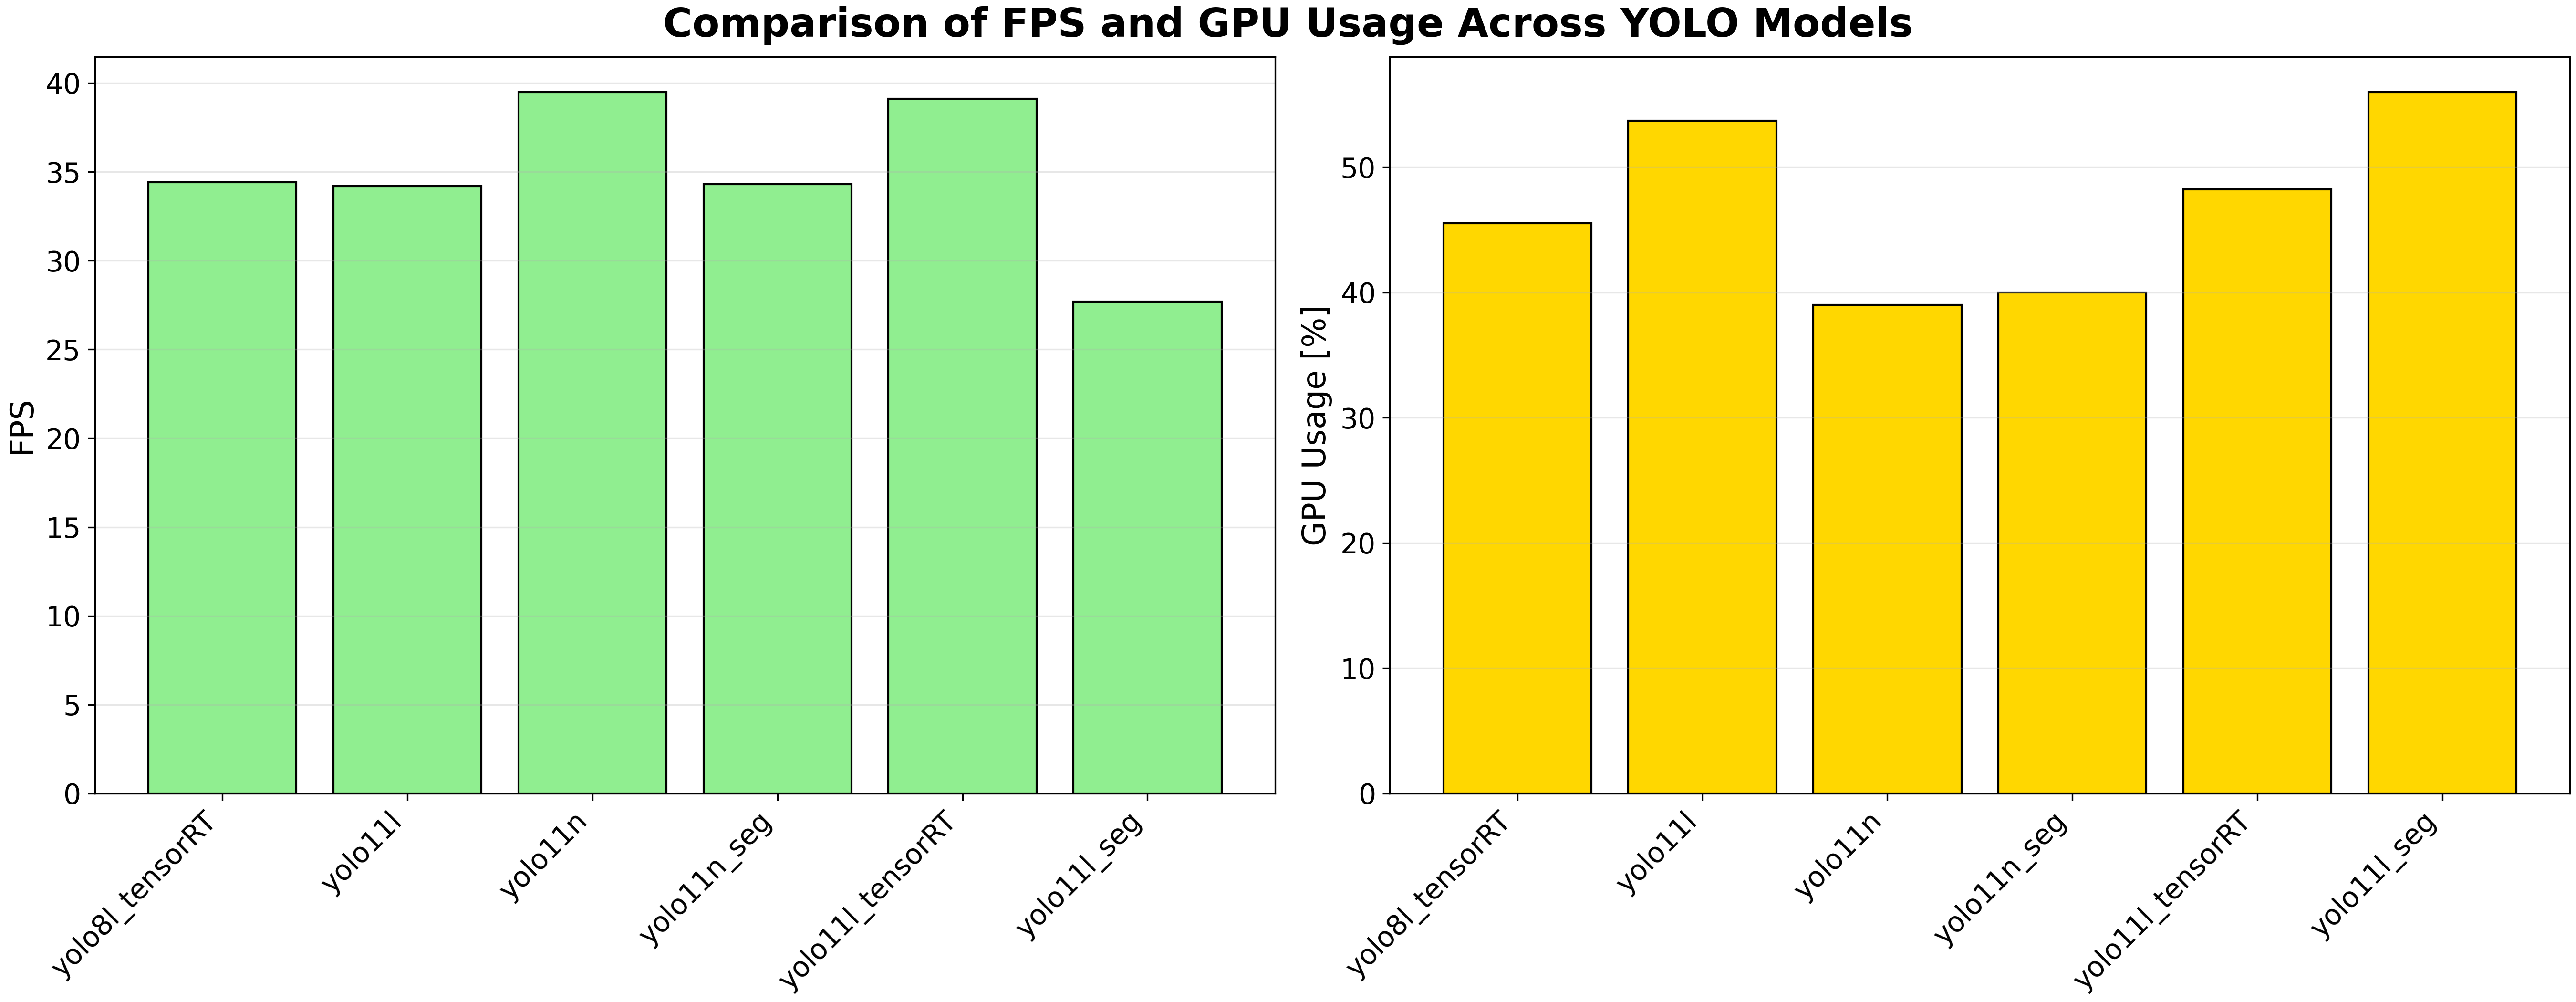
\includegraphics[width=\textwidth]{images/yolo_comparison.png}
	\caption{FPS and GPU usage analysis of YOLO models on the laptop with an average of 5.5 static and 1.1 active objects (objects in motion) captured over 1750 frames.}
	\label{fig:yolo_comparison}
\end{figure*}

\begin{figure}[!t]
	\centering
	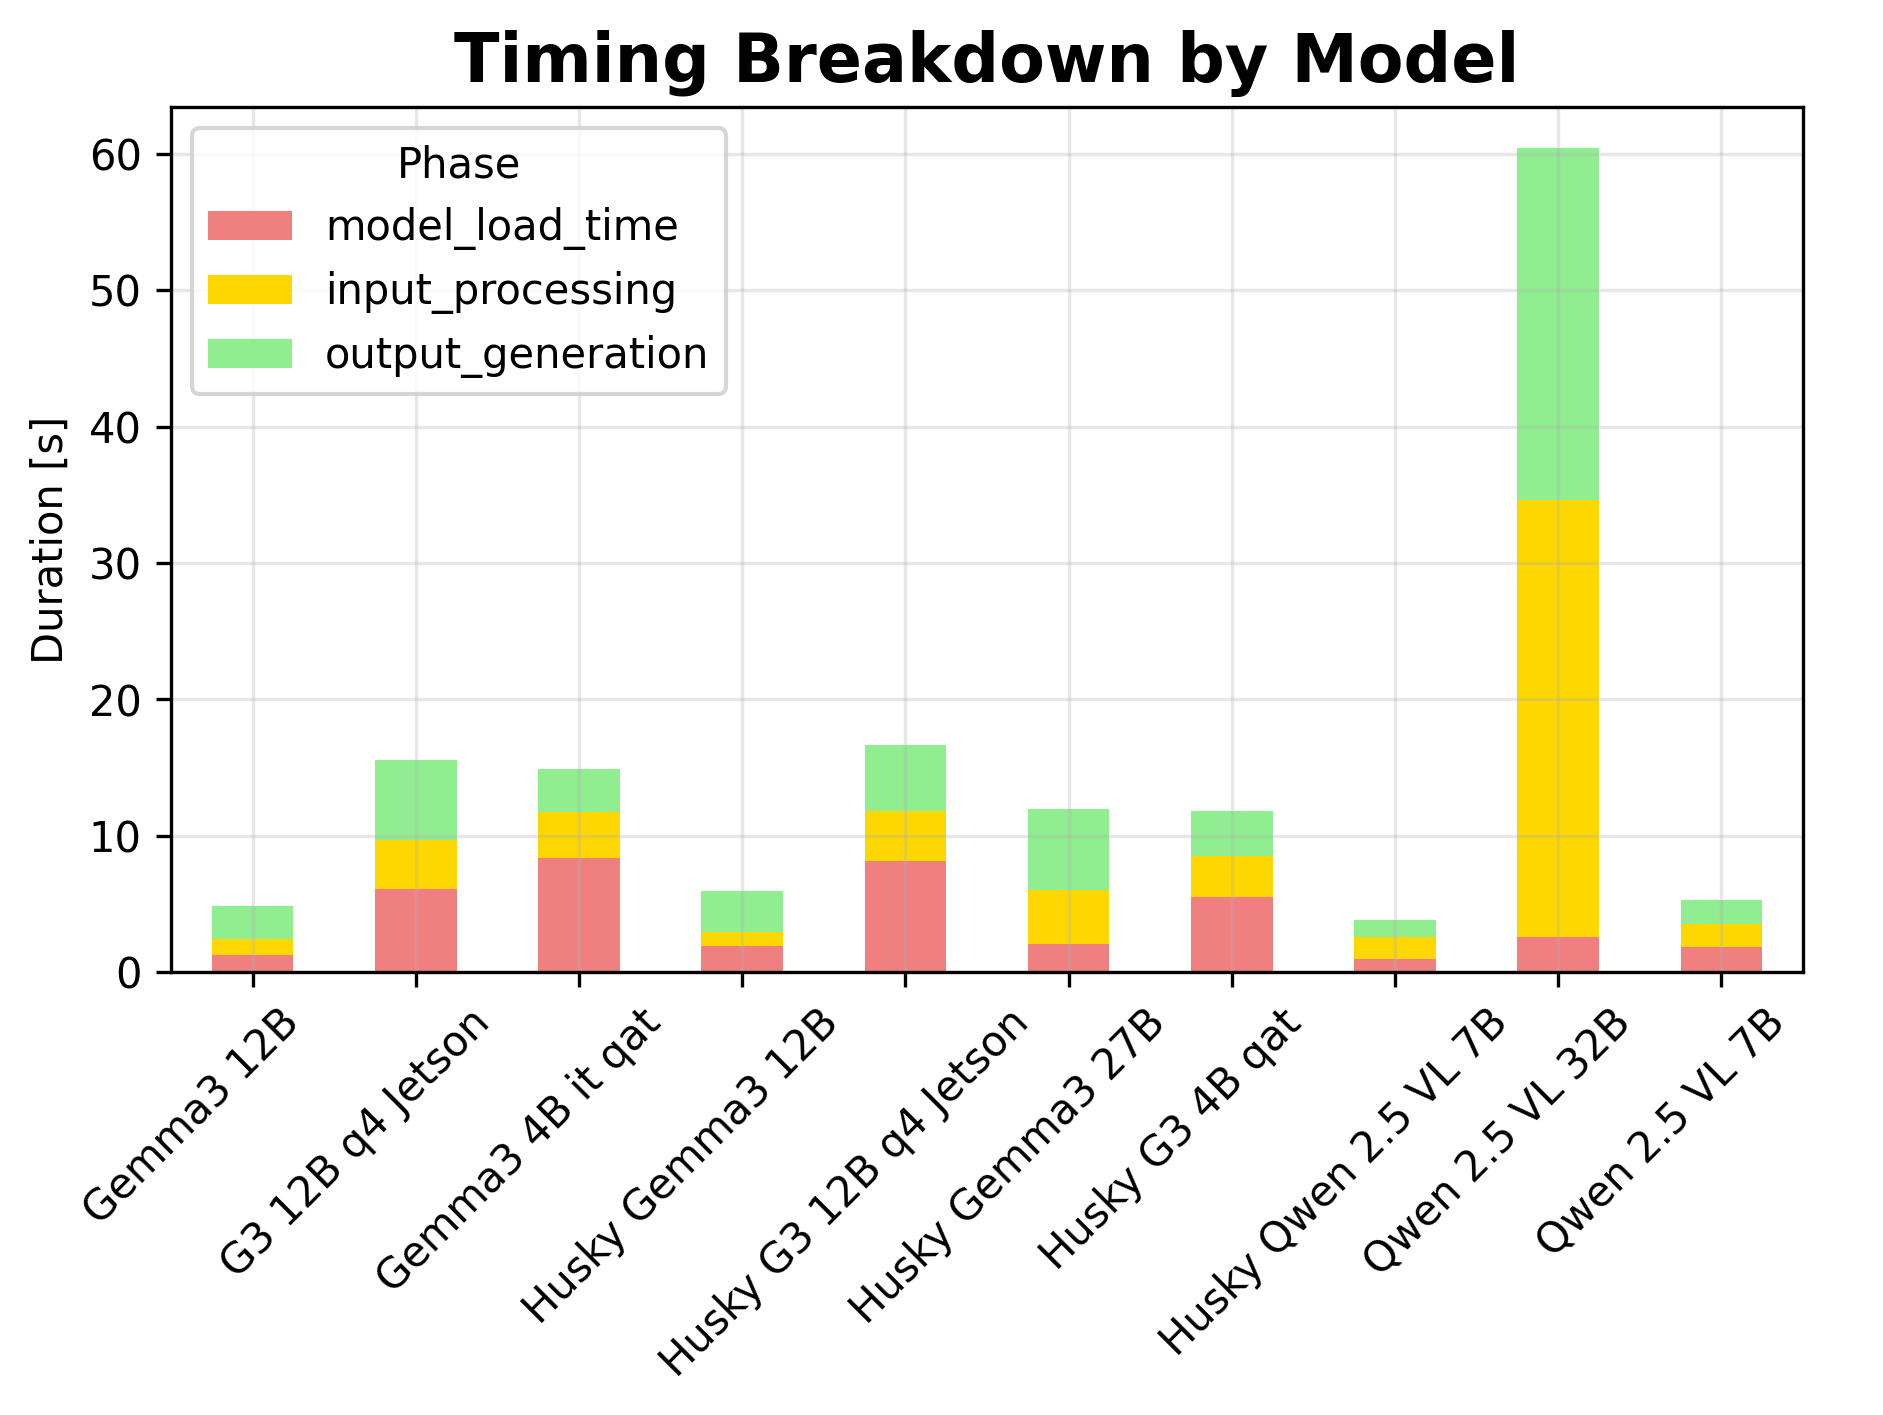
\includegraphics[width=8.5cm]{images/timing_breakdown.png}
	\caption{Timing breakdown of Gemma 3 and Qwen 2.5 VL models based on size. The suffix "Husky" indicates that the model has been modified using modelfile parameters and adapted to our application. Abbreviations: "G3" = Gemma 3, "it qat" = instruction-tuned and Quantization-Aware Training, "Q4" = 4-Bit quantization.}
	\label{timing_breakdown}
\end{figure}

\begin{figure}[!htbp]
	\centering
	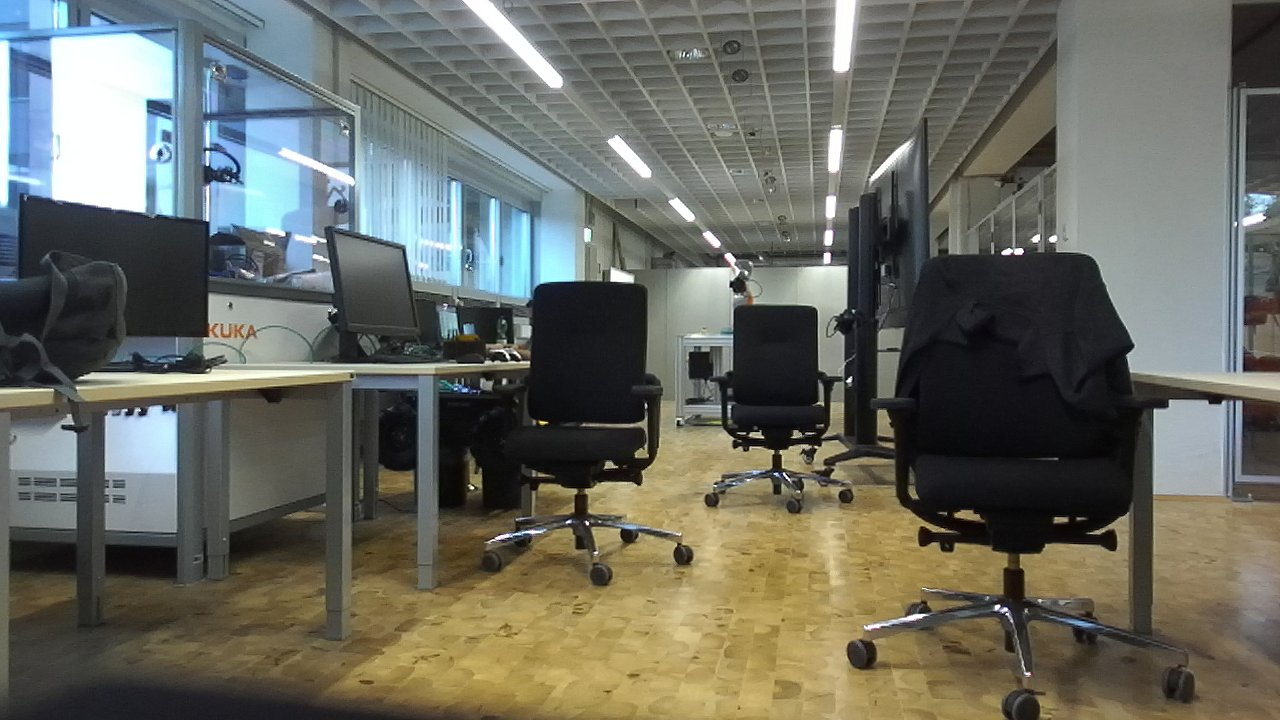
\includegraphics[width=\columnwidth] {images/lab.jpg}
	\caption{Qualitative assessment of Gemma 3 12B scene description capability. The model integrates real-time object detection data to generate a natural language representation of the robot's environment for assistive navigation. The scene description generated by a Gemma 3 12B model with spatial object data, reads as follows: \textit{"You are in a room, presumably an
			office. Directly in front of you,
			about 1.8 meters away and slightly to
			the left, is a screen. To your right,
			about 2.5 meters away, is a chair. To
			your left, about 3.7 meters away, is
			another chair. A little further ahead,
			about 4 meters away and to your left,
			is another screen. To your right,
			about 5 meters away, is another chair.
			Be aware of the chairs and screens as
			potential obstacles. The floor appears
			to be level."} This response was originally generated in German.}
	\label{mllm_scene_lab}
\end{figure}


\begin{figure}[bh!]
	\centering
	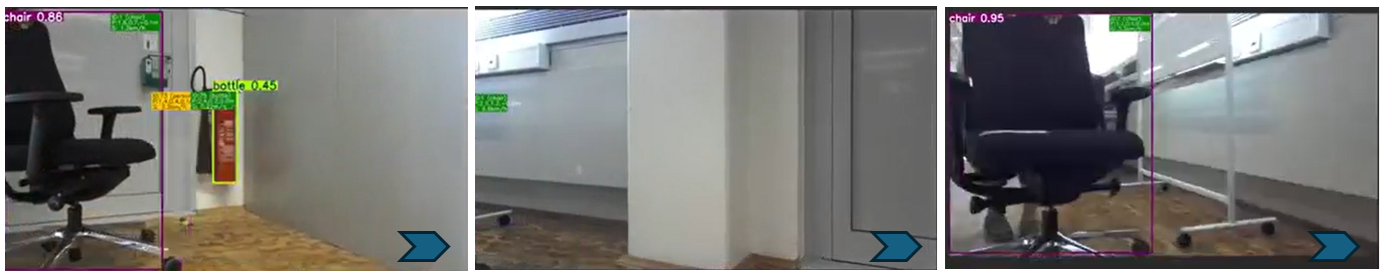
\includegraphics[width=0.9\columnwidth]{images/reentrance.png}
	\caption{Memory recall analysis: User queries a chair that has left the scene, and the SG correctly retrieves its past and current attributes from memory.}
	\label{renentrance} %\label{SGmemory}
\end{figure}

\subsection{Performance of MLLM-Based  Scene Understanding}
\label{subsec:sceneunderstanding}



Fig.~\ref{timing_breakdown} presents the inference time of several Gemma~3 and Qwen~2.5~VL models for generating scene descriptions from object data. The measurements were recorded using Ollama logs, which contain metadata such as timestamps, unique identifiers (linking images and audio files to analysis logs), the model used for scene interpretation, and the number of input and output tokens. In all experiments, the same scene was evaluated across different models. The total response time-from the user request to the generated scene description-was divided into three components: model loading time, input processing time, and output generation time transmitted from the server to the client device running \textit{pAIrSEEption}. The runtime analysis shows that model size is the primary factor influencing system responsiveness. Very large models such as Qwen~2.5~VL~32B require more than 60~seconds to process a request and are therefore unsuitable for assistive applications given the server hardware constraints (Intel i9-13900KF CPU, RTX~A5000 GPU, and 128\,GB RAM). Smaller models such as Husky Qwen~2.5~VL~7B and Gemma~3~12B produce responses in under 6~seconds, making them suitable for near real-time operation. When running directly on the Jetson platform (e.g., G3~12B~Q4 Jetson), the initial model loading time (\textit{model\_load\_time}) becomes the main latency bottleneck. The results also show that application-specific Husky customizations implemented via modelfiles introduce no measurable performance overhead. In practice, lightweight models with 7B or 12B parameters provide the best balance between performance and responsiveness. On Jetson systems, keeping the model resident in memory can further reduce loading delays. Fig.~\ref{mllm_scene_lab} illustrates a laboratory scene described by the Gemma~3~12B model. The generated output demonstrates strong spatial awareness and semantic coherence. By combining YOLO-based detections with ZED-derived depth information, the model effectively translates metric coordinates into natural language descriptions. The obstacles are ordered chronologically by distance (1.8\,m to 5.0\,m) without explicit instruction. Detected static objects are correctly identified as potential obstacles, indicating effective reasoning within the task-related layer of the SG. Additionally, the model remarks on global scene properties such as the floor condition,  stores and recalls last known attributes (e.g., identity, location, and task relevance) of objects  after occlusion/re-entrance (see \cref{renentrance}), demonstrating persistent interpretation  beyond  YOLO preprocessing stages. This behavior supports a human-centered design that prioritizes user safety and situational awareness. Though focusing on locally hosted models,  experiments were also conducted with larger cloud-based MLLMs via OpenRouter (e.g., Llama~4~Scout/Maverick and Gemini~2), which produced similarly accurate scene descriptions.


\begin{figure}[ht]
	\centering
	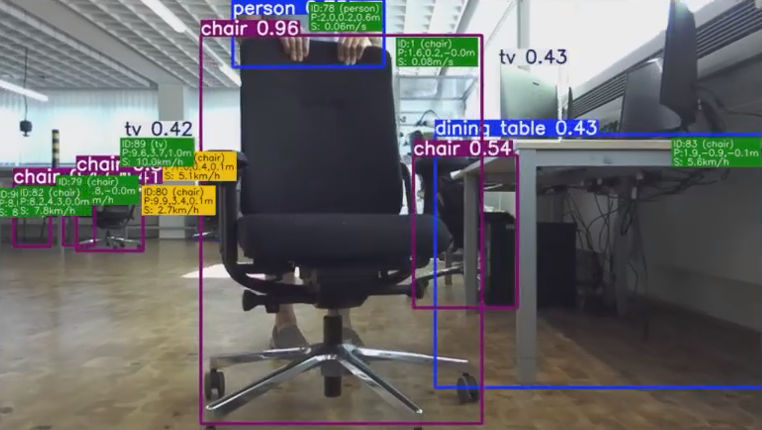
\includegraphics[width=\columnwidth]{pic/mental.png}
	\caption{\textit{Indoor} scene from the viewpoint of the robot mounted camera. Semantic perception of objects for structured description of the {indoor} environment by the mobile robot as SG-based mental model. The robot reasons over this graph using  MLLM and makes the decision to track the moving chair in response to the verbal human instruction and persistent context.}
	\label{mental1}
\end{figure}



\subsection{Usability Studies}
We conducted a total of two usability studies:
In the first phase, we conducted a usability study with a group of end users of the implemented framework, who tested the robot system on-site in a practical setting. To complement this, we also included a video-based assessment of recorded interactions with participants from or based in Africa, Asia and Europe in the second phase. Because of geographical distance and limited remote access, hands-on testing was not feasible for these participants. However, their input allowed us to capture perspectives shaped by different cultural contexts and local needs. While not equivalent to direct interaction with the  system, the video-based approach revealed additional insight into how the system is perceived across contexts.
%The following section first presents and analyzes the on-site field study. The design and analysis of the second video-based study follows thereafter.

\subsubsection{Phase 1: On-site Setup Expert Evaluation}

For the on-site testing, nine participants  with  engineering backgrounds (undergraduate and graduate students, two females and seven males) interacted with the Husky mobile robot indoors (see \cref{mental1}) and outdoors (see \cref{mental2}) using German voice commands (e.g., ``Folge Stuhl'' = ``Follow chair'', ``Folge Person~1'' = ``Follow person~1''). After a brief introduction to the GUI and system functionality, participants verbally instructed the robot to follow selected targets over distances chosen by themselves. Voice commands could also be used to stop navigation or switch to a different target. During operation, the robot provided audio feedback describing its objectives, state, and actions. After completing the interaction, participants anonymously evaluated their experience through a survey.
To evaluate the usability of the system, particularly voice control and object tracking (following a target with the mobile robot), a survey was conducted consisting of nine Likert-scale items (rated from 1 to 5) and three open-ended questions. The items were structured as follows:

\begin{itemize}[leftmargin=*]
	\item \textbf{Voice Control:} 
	\begin{enumerate}[label=Q\arabic*:, series=survey, widest=Q12, leftmargin=*]
		\item Ease of issuing instructions.
		\item Reliability of command recognition  and execution despite evolving tasks.
		\item Necessity of repetitions (negative item*). 
	\end{enumerate}
	
	\item \textbf{Context-Aware Object Tracking:} 
	\begin{enumerate}[label=Q\arabic*:, resume=survey, widest=Q12, leftmargin=*]
		\item Accuracy of object identification  in various contexts.
		\item System response time to navigation instructions. 
		\item Frequency of losing the target in evolving tasks (negative item*). 
	\end{enumerate}
	
	\item \textbf{User Experience:} 
	\begin{enumerate}[label=Q\arabic*:, resume=survey, widest=Q12, leftmargin=*]
		\item Overall ease of understanding and using the robot. 
		\item Perceived safety during operation. 
		\item Intention to use the system in real-world applications. 
	\end{enumerate}
	
	\item \textbf{Qualitative Feedback (Open-ended):} 
	\begin{enumerate}[label=Q\arabic*:, resume=survey, widest=Q12, leftmargin=*]
		\item Positive aspects of system operation. 
		\item Suggestions for improving user experience$\slash$comfort.
		\item Proposed additional functions or commands. 
	\end{enumerate}
\end{itemize}

\begin{figure}[ht]
	\centering
	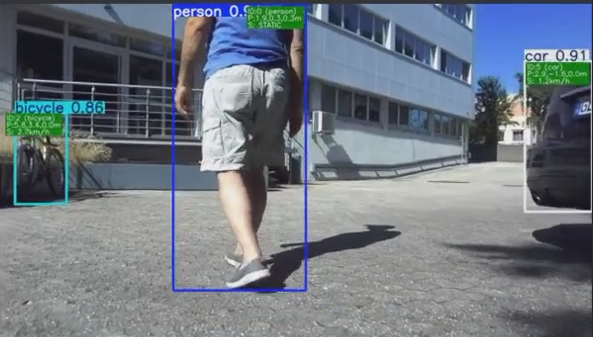
\includegraphics[width=\columnwidth]{pic/mental2.png}
	\caption{\textit{Outdoor} scene from the viewpoint of the robot mounted camera. The robot semantically understands the {outdoor} environment. It follows its human teammate {from behind} while providing real-time, natural-language insights into the usefulness of surrounding objects, facilitating smart mobility. These include obstacles (e.g., cars) and items relevant for active transportation (e.g., bicycles). By reasoning over relative pose, object affordances, and user needs, the robot with a \textit{task-grounded SG} assesses reachability and can guide its teammate toward cycling. This supports a vision of future society where robots seamlessly assist daily  activities and empower human self-determination.}
	\label{mental2}
\end{figure}


The questions $Q_{i,\, i \in \{1,\dots,9\}}$ were rated by participants (P1--P9) on a five-point scale, where 1 indicates the lowest/worst rating and 5 the highest/best rating. For questions Q3 and Q6 (negative items), responses were reverse-coded for statistical analysis (1 = best, 5 = worst). For each quantitative question (Q1--Q9), the mean $\bar{x}$ and the sample standard deviation (SD) $s$ were calculated. %Since participant P5 skipped question Q3, $n = 8$ was used to compute the mean and standard deviation for that item.

\subsubsection{Results and Discussion of Phase I}
\begin{table}[!b]
	\centering
	\caption{Quantitative Results of the Usability Evaluation ($N=9$) featuring Mean Score $\bar{x}$ and Sample Standard Deviation $s$. Scoring: 5 = highest/best, 1 = lowest/worst.
		*Negative questions: lower values indicate better performance.}
	\label{tab:user_study_results}
	\setlength{\tabcolsep}{3.5pt} 
	\begin{tabular}{|l|c|c|c|c|c|c|c|c|c|}
		\hline
		\textbf{Participant} & \textbf{Q1} & \textbf{Q2} & \textbf{Q3*} & \textbf{Q4} & \textbf{Q5} & \textbf{Q6*} & \textbf{Q7} & \textbf{Q8} & \textbf{Q9} \\ \hline
		P1 & 4 & 4 & 3 & 5 & 4 & 1 & 4 & 5 & 4 \\ \hline
		P2 & 4 & 4 & 3 & 5 & 5 & 1 & 4 & 5 & 4 \\ \hline
		P3 & 5 & 5 & 1 & 4 & 5 & 2 & 5 & 5 & 5 \\ \hline
		P4 & 5 & 5 & 1 & 5 & 5 & 2 & 5 & 5 & 5 \\ \hline
		P5 & 5 & 5 & $-$ & 4 & 5 & 1 & 5 & 5 & 5 \\ \hline
		P6 & 5 & 5 & 1 & 5 & 5 & 1 & 4 & 4 & 5 \\ \hline
		P7 & 5 & 4 & 2 & 5 & 4 & 3 & 4 & 4 & 3 \\ \hline
		P8 & 4 & 5 & 1 & 5 & 4 & 1 & 5 & 5 & 2 \\ \hline
		P9 & 5 & 4 & 2 & 5 & 4 & 2 & 5 & 4 & 5 \\ \hline \hline
		\textbf{Mean} $\bar{x}$ & \textbf{4.67} & \textbf{4.56} & \textbf{1.75} & \textbf{4.78} & \textbf{4.56} & \textbf{1.56} & \textbf{4.56} & \textbf{4.67} & \textbf{4.22} \\ \hline
		\textbf{SD} $s$ & \textbf{0.50} & \textbf{0.53} & \textbf{0.89} & \textbf{0.44} & \textbf{0.53} & \textbf{0.73} & \textbf{0.53} & \textbf{0.50} & \textbf{1.09} \\ \hline
	\end{tabular}
	\vspace{1ex}
\end{table}

The quantitative results in Table~\ref{tab:user_study_results} indicate a high level of user satisfaction across all evaluated categories. In particular, the ease of issuing voice commands and the perceived safety during robot operation received high ratings ($\bar{x}_{Q1,Q8} = 4.67$, $s_{Q1,Q8} = 0.50$). The accuracy of object identification achieved the highest mean score ($\bar{x}_{Q4} = 4.78$) with the lowest standard deviation ($s_{Q4} = 0.44$), indicating both strong performance and high agreement among participants.

High ratings were also observed for command recognition reliability, system response time, and overall usability ($\bar{x}_{Q2,Q5,Q7} = 4.56$), suggesting that the tracking behavior was perceived as predictable and safe. Participants also expressed a strong willingness to use such a system in real-world applications ($\bar{x}_{Q9} = 4.22$). Conversely, the low scores for the necessity of command repetition ($\bar{x}_{Q3} = 1.75$) and the frequency of losing  tracked   previously unseen targets and task contexts ($\bar{x}_{Q6} = 1.56$) further indicate that both the voice control and object tracking performed reliably \textcolor{black}{with a task success rate of $100\%$ end-to-end and without taking re-identification (Re-ID) into account.} The low standard deviations across items suggest a strong consensus among participants.

However, this study has several limitations. All participants had engineering backgrounds and were undergraduate or graduate students, reflecting a relatively high level of technical familiarity and intrinsic interest in robotics. As such, usability and acceptance are likely to differ for non-expert users, particularly in real-world societal contexts. Furthermore, the small sample size ($N=9$) limits generalization and positions this study as a pilot evaluation. Despite these limitations, the findings demonstrate the framework’s potential to enable context-aware, intuitive, and task-grounded human–robot interaction.

Future studies should involve visually impaired users to evaluate the practical usefulness of the generated scene descriptions (Fig.~\ref{mllm_scene_lab}) for independent navigation. Moreover, although object tracking performance was rated highly in the current controlled environment, future work should investigate more cluttered or unstructured settings where the probability of losing the target (Q6) may increase.

Qualitative feedback (Q10-Q12) revealed both strengths in operational performance and areas for improvement. The system’s precision, responsiveness, interface clarity, and stable distance maintenance during following tasks were consistently highlighted, while smoother turning behavior and broader language support were identified as key areas for enhancement. Although the current architecture employs \textit{faster-whisper}~\cite{fasterwhisper} for automatic language recognition (input), TTS output remains limited to German. Given the multilingual capabilities of the integrated MLLMs, extending language support is a key direction for future development.

Further recommendations included improvements in object Re-ID \textcolor{black}{from a current  identification accuracy of $75\%$}, obstacle detection, and voice command guidance, as well as additional functionalities such as reverse driving, 180$^\circ$ turning, robotic arm integration, and inter-robot communication. The need for fallback mechanisms to handle voice-signal loss and for additional communication modalities to enhance robustness was also highlighted. Overall, these findings indicate that the proposed system lowers the barrier to human-robot teaming and demonstrates strong potential for service robotics in societal environments.

\subsubsection{Phase 2: Remote and Global  Video-based Study}
The second group comprised 10 additional participants without prior robotics experience, representing a broad demographic spectrum (ages 8–74 years, mean $\bar{x}_{age} = 43.9$, five male and five female) across Africa, Asia, and Europe. In this phase, participants evaluated the system based on two videos: one showing verbal human-robot interaction and demonstrating navigation and object-tracking capabilities in an indoor environment, and the other demonstrating human-following with assistance and guidance in an outdoor environment. The qualitative assessment was structured around three condensed questions, consistent with Phase I: interaction quality, trust in navigation and system behavior, and practical utility.

The results indicate a comparable level of perceived usefulness to that observed in Phase I. Nine participants described the interaction as natural, reflecting overall positive perceptions, while one participant did not respond. High levels of trust were reported in both navigation and conversational capabilities, with particularly strong confidence among younger European participants. However, two participants from Africa emphasized the need to improve technical reliability in dynamic or structurally challenging environments (e.g., complex road conditions or flooded areas).

These findings highlight the importance of evaluating SG-based semantic understanding under diverse environmental and seasonal conditions to further assess the robustness of the system’s reasoning and navigation. Participants also identified practical applications in logistics, agriculture, and retail. Notably, the system received high acceptance among  participants, particularly in the context of elderly care and daily assistance in African settings. Feedback from Africa and Asia further underscores the importance of supporting local languages to facilitate adoption, improve global accessibility and user experience. Overall, the second-phase study indicates a high potential for social acceptance, even among non-expert users.

\section{Conclusion}\label{conclusion}

This work introduced a framework for SGG that integrates precise 3D sensor data with the semantic reasoning capabilities of MLLMs for mobile robotics. By transforming structured metric object data into natural language representations, the proposed approach bridges perception and semantic understanding, enabling both human interpretability and actionable awareness of the environment. The resulting SGs support intuitive navigation, assistance, and guidance, making robotic behavior more transparent and accessible, particularly for users with limited visual perception. Experimental results demonstrate that grounding MLLM reasoning in sensor data leads to factually consistent scene interpretations, while user studies confirm high perceived reliability, safety, and social acceptance. Overall, this work advances toward extended, human-centered robot intelligence, in which robots can reason about their environment and communicate this understanding at a high level to support inclusive and meaningful human–robot collaboration. The proposed framework empowers users to better understand, guide, and collaborate with robotic systems in real-world environments, paving the way for a more inclusive and capable robotized society. Toward this vision, we move closer to robots that are task-grounded, memory-augmented, and capable of introspection. These robots can combine perception, task context, and interaction history to generate human-interpretable explanations of their environment and behavior.

\section*{Acknowledgments}
The authors would like to thank Mr. N. Mahr and Mr. N. Schenkel for their support in conducting the task grounding and memory augmentation study, and Mr. A. Koennecke for his support with robot control. The authors also thank all participants for their time and valuable feedback.

During the preparation of this manuscript, the author(s) used the GPT-5.3 model to improve the language and readability. After using this tool, the authors reviewed and edited the content as necessary. 
\bibliographystyle{IEEEtran}
\bibliography{references}


%\newpage





\vfill

\end{document}


